% last updated in April 2002 by Antje Endemann
% Based on CVPR 07 and LNCS, with modifications by DAF, AZ and elle, 2008 and AA, 2010, and CC, 2011; TT, 2014; AAS, 2016

\documentclass[runningheads]{llncs}
\usepackage{graphicx}
\usepackage{amsmath,amssymb} % define this before the line numbering.
\usepackage{ruler}
\usepackage{multirow}
\usepackage{booktabs}
\usepackage{threeparttable}

\usepackage{pifont}
\usepackage{color}
\usepackage[width=122mm,left=12mm,paperwidth=146mm,height=193mm,top=12mm,paperheight=217mm]{geometry}
\usepackage[pagebackref,breaklinks,colorlinks,citecolor=blue]{hyperref}
\begin{document}
% \renewcommand\thelinenumber{\color[rgb]{0.2,0.5,0.8}\normalfont\sffamily\scriptsize\arabic{linenumber}\color[rgb]{0,0,0}}
% \renewcommand\makeLineNumber {\hss\thelinenumber\ \hspace{6mm} \rlap{\hskip\textwidth\ \hspace{6.5mm}\thelinenumber}}
% \linenumbers
\pagestyle{headings}
\mainmatter
\def\ECCV16SubNumber{13487}  % Insert your submission number here
\newcommand{\methodname}{TextComp} 
\title{TextComp: Text-Guided Learning for Compressed Video Action Recognition} % Replace with your title

\titlerunning{ECCV-26 submission ID \ECCV16SubNumber}

\authorrunning{ECCV-26 submission ID \ECCV16SubNumber}

\author{Anonymous ECCV submission}
\institute{Paper ID \ECCV16SubNumber}


\maketitle

\begin{abstract}
Compressed video action recognition operates directly on codec-domain representations such as I-frames, motion vectors, and residuals, offering high computational efficiency without full decoding. However, due to the temporal sparsity of I-frames and the coarse, noisy nature of motion vectors and residuals, existing approaches often rely on carefully designed architectures and modality-specific learning strategies to extract discriminative representations from these heterogeneous signals. With the rapid advancement of Vision-Language Models (VLMs), textual information has demonstrated strong semantic expressiveness and the ability to provide high-level guidance for visual understanding. 
Motivated by this, we propose TextComp, the first framework to introduce text-guided semantic navigation into compressed video modeling. Instead of viewing textual information as a simple label, TextComp treats it as a semantic anchor that guides the model to "identify" relevant signals within the fragmented compressed stream. We leverage a Large Language Model (LLM) to decompose action labels into multi-faceted semantic attributes—covering appearance, motion style, and contextual cues.
To effectively harness these priors, we design an Instance-Aware Dynamic Fusion (IADF) module. Rather than performing static integration, IADF employs cross-modal attention to use these textual attributes as "navigators," adaptively modulating and filtering the heterogeneous codec signals (I, MV, Res) based on the specific semantic requirements of each video instance. This approach allows the model to selectively focus on discriminative motion patterns or appearance cues even when the visual signal is heavily degraded.
Extensive experiments across four benchmark datasets demonstrate that TextComp consistently outperforms prior state-of-the-art approaches.
\keywords{Compressed Video, Action Recognition, Vision-Language Models}
\end{abstract}

\section{Introduction}
\label{sec:intro}

With the increasing demand for scalable and efficient video understanding, compressed video action recognition has emerged as a compelling paradigm. By directly leveraging codec-domain signals—such as I-frames (IF), motion vectors (MV), and residuals (Res)—without full decoding, this approach significantly reduces computational overhead and memory usage, making it ideal for real-time and large-scale scenarios.

\begin{figure}[t!]
\centering 
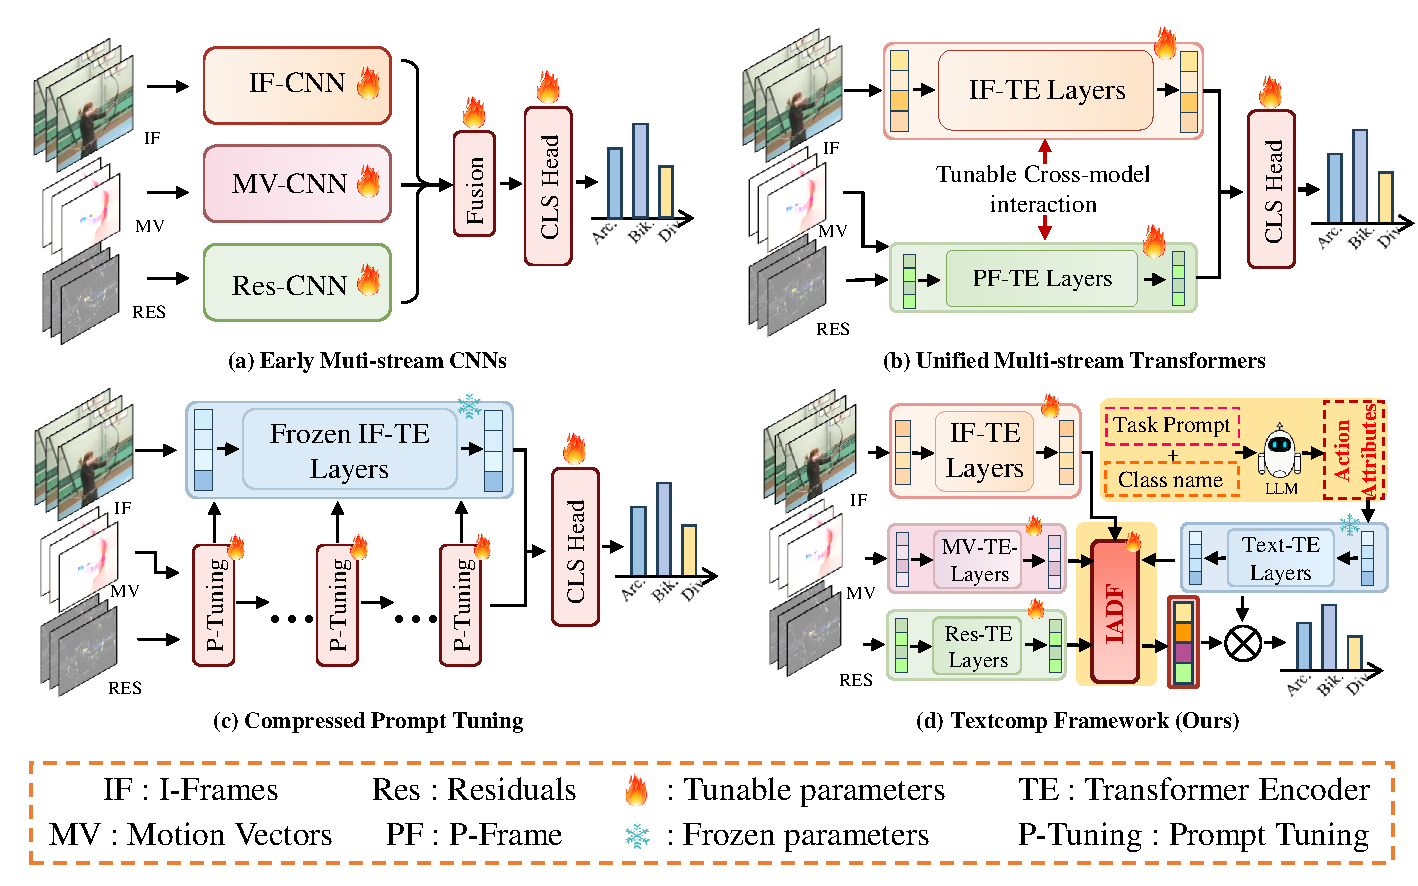
\includegraphics[width=\columnwidth]{figure/figure1-s.pdf}
\caption{Comparison of architectural paradigms for compressed video action recognition. (a) Early Multi-stream CNNs use separate branches for I-frames (IF), motion vectors (MV), and residuals (Res). (b) Unified Multi-stream Transformers introduce cross-modal interaction between IF and PF encoders. (c) Compressed Prompt Tuning applies parameter-efficient tuning to compressed videos. (d) TextComp (Ours) introduces a text-guided approach: an LLM generates action attributes which are then used by the Instance-Aware Dynamic Fusion (IADF) module to adaptively guide the integration of compressed modalities.}
\label{fig:type}
\end{figure}

Despite its efficiency, the compressed domain faces a fundamental challenge: inherent semantic sparsity. As illustrated in Fig.~\ref{fig:type}, the development of compressed video architectures to address this limitation can be broadly categorized into three paradigms.
(i) \cite{battash2020mimic,huang2019flow,hu2023efficient,huo2021compressed,simonyan2014two} apply multi-branch CNNs to extract features from individual modalities (IF, MV, and Res) through separate streams, which are then fused at the decision or feature level to deliver the final results Fig.~\ref{fig:type}(a); (ii) \cite{chen2022mm,CFM-Net-li2025interactive,guo2026hierarchical}  introduce unified multi-stream Transformers that incorporate cross-modal interaction modules to capture the intrinsic correlations between IF and P-frame (MV and Res) encoders, aiming for a more cohesive representation Fig.~\ref{fig:type}(b); (iii) \cite{li2023compressed} employ parameter-efficient tuning strategies, such as prompt tuning or adapters, to adapt large-scale frozen pre-trained models to the specific characteristics of codec-domain signals Fig.~\ref{fig:type}(c).

However, since these methods rely solely on fragmented and noisy visual inputs, they often struggle to distinguish subtle action patterns from codec-induced noise. The lack of high-level semantic guidance leaves these models constrained by the "semantic gap" between raw bitstreams and complex human actions.

Recent advancements in Vision-Language Models (VLMs) suggest that textual information can provide powerful high-level semantic cues to complement visual perception. While this vision-language synergy has flourished in the RGB domain, its potential in compressed video remains largely untapped. We argue that semantic guidance is even more critical in the compressed domain: when visual signals are sparse or coarse, linguistic priors can act as a "navigator," directing the model to identify and focus on relevant signal fragments across the heterogeneous I, MV, and Res streams.

Motivated by this, we propose TextComp (Fig.~\ref{fig:type}d), the first framework to integrate text-guided semantic navigation into compressed video modeling. Instead of using simple class labels, TextComp leverages a Large Language Model (LLM) to decompose actions into multi-faceted semantic attributes. These attributes are specifically designed to correspond with the characteristics of codec signals: for instance, appearance attributes provide anchors for I-frames, while motion-style attributes guide the extraction of dynamics from motion vectors.

To effectively bridge these modalities, we introduce an Instance-Aware Dynamic Fusion (IADF) module. Unlike previous static fusion or purely visual interactions shown in Fig.~\ref{fig:type}(a-c), IADF employs cross-modal attention to use visual features as queries to retrieve relevant semantic cues from textual attributes. This allows the model to adaptively modulate and filter compressed features on an instance-by-instance basis. By "querying" the video features with semantic attributes, IADF achieves an optimal, instance-specific integration, effectively highlighting discriminative patterns even within heavily degraded visual signals.

The main contributions of this paper are:
\begin{itemize}
\item We introduce TextComp, establishing a new paradigm for semantically enriched representation learning in the compressed video domain through text-guided navigation.
\item We propose a label-guided semantic attribute decomposition strategy, using LLMs to provide multi-dimensional guidance (appearance, motion, and context) tailored to the diverse characteristics of I, MV, and Res signals.
\item We design an Instance-Aware Dynamic Fusion (IADF) module that leverages cross-modal attention to achieve adaptive, instance-level modulation of compressed modalities based on semantic intent.
\item TextComp achieves state-of-the-art performance on four public benchmarks, validating the effectiveness of semantic guidance in the compressed domain.
\end{itemize}


\section{Related Work}
\label{sec:related_work}
\subsection{Action Recognition in Raw Videos}
Action recognition research has focused on effectively extracting spatiotemporal information from video data. Traditional methods primarily operate in the pixel domain, with Two-Stream Networks \cite{simonyan2014two} pioneering the use of RGB frames for appearance features and optical flow for motion cues. Building upon this, various improvements have been proposed, including Temporal Segment Networks \cite{wang2016temporal}, dense dilated networks \cite{xu2019dense}, and spatiotemporal factorized convolutions. Recent efforts like TCM \cite{liu2022motion} leverage low-level features, while transformer-based approaches \cite{piergiovanni2023rethinking} address challenges in low FPS sampling and per-frame modeling.

Despite these advances, pixel-domain methods face fundamental limitations. Optical flow estimation introduces massive computational overhead, severely limiting real-time performance on resource-constrained devices. Frame-wise decoding and motion recomputation further exacerbate inefficiencies, while discrete RGB sampling poses challenges in capturing long-range temporal dependencies, making it difficult to balance accuracy and efficiency in practical deployment.

Alternative approaches using semantic \cite{tu2019semantic,shen2022fexnet,luo2022dense}, skeleton \cite{tu2022joint,xiong2023human,liu2023novel,shu2023multi,xu2023spatiotemporal,xu2023pyramid}, and RGBD data \cite{cheng2022cross} enhance foreground extraction through additional modalities. However, these introduce extra hardware or computational costs, limiting practical applicability.

In contrast, our work operates directly on compressed video streams, avoiding expensive optical flow estimation and full frame decoding, enabling significant efficiency gains while maintaining competitive accuracy for resource-constrained scenarios.

\subsection{Action Recognition in Compressed Videos}
\label{subsec:compressed_learning}
\begin{figure*}[t!]
\centering 
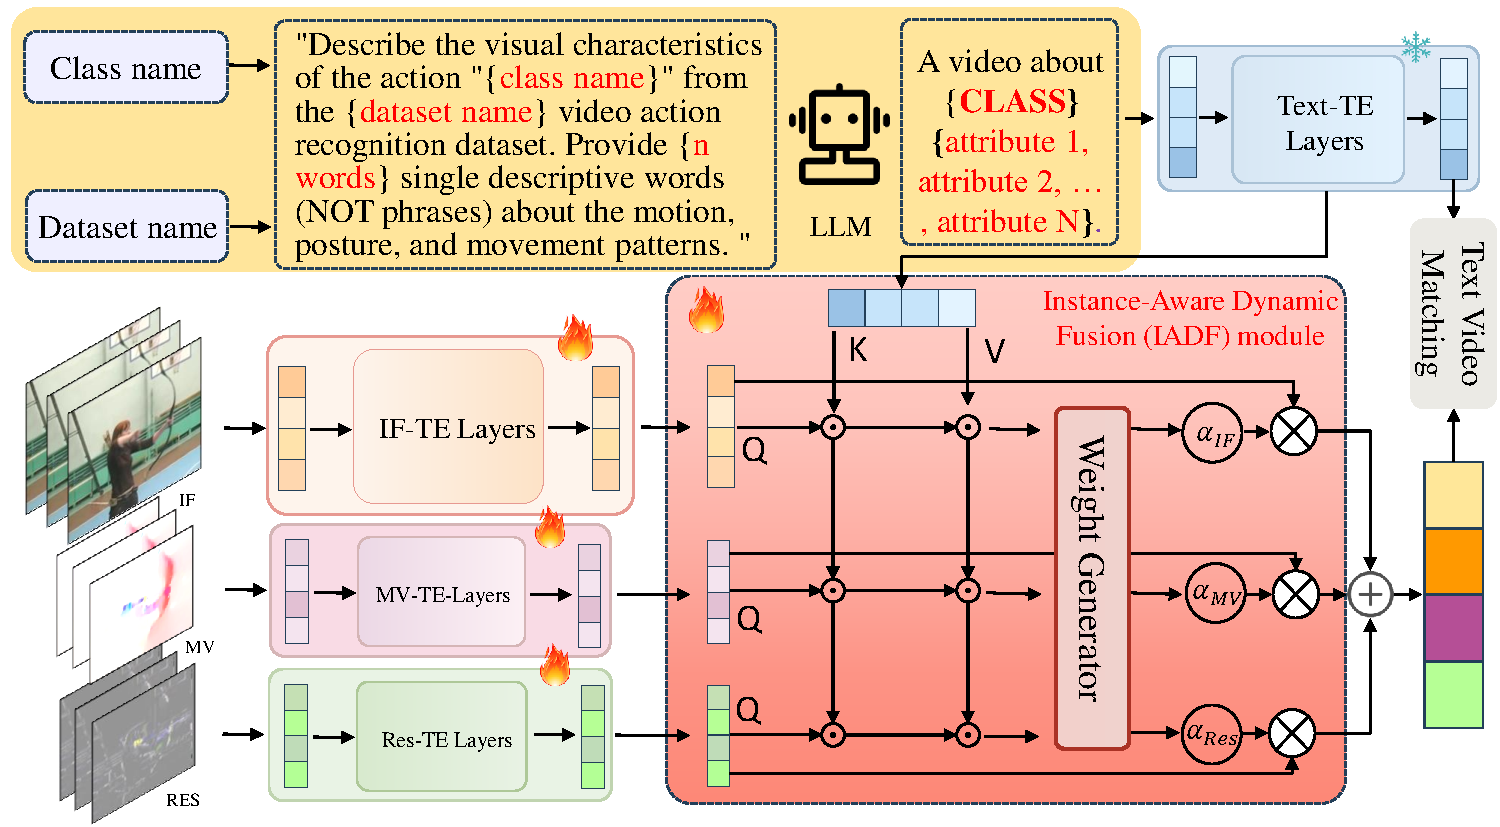
\includegraphics[width=\textwidth]{figure/figure2.pdf}
\caption{Overview of the \methodname framework. The visual branch encodes I-frames, motion vectors, and residuals into features. The textual branch generates attribute embeddings that are decomposed into appearance, motion, and interaction semantics. These semantics guide dynamic fusion of visual features for action classification.}
\label{fig:framework}
\end{figure*}
% English
Early approaches sought to improve efficiency by incorporating codec-domain cues—such as motion vectors (MVs) and residuals—as substitutes or auxiliary inputs for optical flow or RGB frames, thereby reducing the need for full decoding and optical flow estimation. For instance, the pioneering work of \cite{zhang2016real} replaced optical flow in two-stream architectures \cite{simonyan2014two} with motion vectors to achieve greater efficiency. While CoViAR \cite{wu2018compressed} first integrated all three modalities into dedicated network branches to fully leverage codec-domain information. Building upon these efforts, subsequent research aimed to further enhance representation quality by alleviating the inherent limitations of compressed data—such as denoising noisy motion vectors \cite{cao2019compressed} or generating flow-like MVs through generative adversarial networks (GANs) \cite{shou2019dmc}. Beyond data refinement, model architectures were also increasingly customized for codec-domain processing, exemplified by Slow-I-Fast-P networks \cite{li2020slow} that separate intra- and inter-frame dynamics, and Transformer-based designs like MM-ViT \cite{chen2022mm} that employ factorized attention to capture modality interactions more effectively. More recently, self-supervised learning paradigms have been introduced to exploit the inherent structure of compressed videos—IMRNet \cite{yu2020self}, for example, formulates pretext tasks based on motion statistics and GOP hierarchies, while other approaches utilize cross-modal guidance within the compressed domain itself \cite{huo2021compressed} to achieve more coherent feature alignment.

% English
While these methods advance compressed video understanding, they often involve designing specialized modules or pretext tasks, limiting generalization or requiring significant training resources. Furthermore, they typically operate solely within the visual (or compressed signal) modality, lacking mechanisms to incorporate high-level semantic guidance from language, which has proven highly effective in the pixel domain.

\subsection{Parameter-Efficient Adaptation of Pre-trained Models}
\label{subsec:peft_adaptation}

% English
The advent of large pre-trained models, including Vision Transformers (ViTs) and Vision-Language Models (VLMs) \cite{radford2021learning,yuan2021florence}, rendered full fine-tuning increasingly impractical for downstream adaptation, thereby driving the emergence of Parameter-Efficient Fine-Tuning (PEFT) solutions. Prompt tuning, specifically, has gained prominence as a more efficient alternative within this PEFT paradigm.

% English
\textbf{Visual Prompt Tuning:} In computer vision, methods like VPT \cite{jia2022visual} introduced learnable prompt tokens into Transformer inputs, demonstrating strong performance with minimal tunable parameters compared to full fine-tuning. Other PEFT strategies for visual models include adding lightweight adapter modules \cite{chen2022adaptformer} or convolutional bypasses \cite{jie2024convolutional}. When applied to the compressed domain, however, directly transferring prompts learned on RGB data or using generic visual prompts often fails due to the significant modality gap. A crucial step forward was CVPT \cite{li2023compressed}, which proposed generating \textit{visual prompts conditioned on the compressed signals} (MVs, Residuals). This showed the potential of domain-aware visual prompting but remained restricted to adapting the visual encoder only.

% English
\textbf{VLM Prompt Tuning:} Prompting has also been extensively explored for adapting VLMs like CLIP \cite{radford2021learning}. Early methods focused on learning continuous prompts in the text embedding space (e.g., CoOp \cite{zhou2022learning}) or conditioning these prompts on image instances (e.g., Co-CoOp \cite{zhou2022conditional}). While successful for uni-modal prompting (either visual like VPT or textual like CoOp), these approaches do not fully leverage the VLM's cross-modal architecture. To address this, multi-modal prompting methods like MaPLe \cite{khattak2023maple} and MMap \cite{xin2024mmap} were developed. They introduce mechanisms to couple and co-optimize prompts in both the vision and language branches, leading to improved performance by better tuning the joint representation space. However, these advanced multi-modal prompting techniques have, to date, been designed for and evaluated on tasks involving \textit{raw pixel data} (images or decoded video frames).

% English
\textbf{Bridging the Gap:} Despite these parallel advancements, a critical gap remains: compressed video understanding methods largely lack semantic guidance from language, while powerful multi-modal VLM prompting techniques are not designed to handle the unique characteristics and modality shift inherent in compressed data. To the best of our knowledge, effectively adapting VLMs using multi-modal prompts generated directly from compressed signals remains an open challenge. Our work, \methodname, addresses this gap by proposing a framework specifically designed for compressed-sensing-based multimodal prompt  generation, aiming to unlock the full potential of VLMs for efficient and semantically rich compressed video understanding.

\section{Methodology}
\label{sec:method}

\subsection{Overview}
\label{sec:baseline}

Recent advances in vision-language models (VLMs), particularly CLIP~\cite{radford2021learning}, have demonstrated remarkable zero-shot and few-shot capabilities in raw video understanding~\cite{wang2021actionclipnewparadigmvideo,ni2022expanding}, leveraging natural language semantics to guide visual feature learning with superior generalization. However, existing compressed-domain methods~\cite{li2023compressed,CFM-Net-li2025interactive} rely solely on visual encoders without textual supervision, limiting their ability to capture high-level semantics. To bridge this gap, we introduce TextComp, the first CLIP-based framework for compressed-domain action recognition, enabling semantic-aware multimodal fusion through vision-language alignment.

As illustrated in Fig.~\ref{fig:framework}, our framework processes visual and textual information in dual parallel branches. For the visual branch, we extract three compressed-domain modalities from the video bitstream: sparse I-frames $\mathbf{F}_{IF}$, motion vectors $\mathbf{F}_{MV}$, and residuals $\mathbf{F}_{Res}$. I-frames are encoded by the pre-trained CLIP visual encoder to obtain $\mathbf{V}_{IF}$, while motion vectors and residuals use lightweight 2-layer encoders initialized from the first and last layers of the CLIP visual encoder, producing $\mathbf{V}_{MV}, \mathbf{V}_{Res}$. This transfers CLIP's visual priors to codec-specific modalities while maintaining efficiency.

For the textual branch, we leverage fine-grained attribute descriptions beyond simple class names to provide richer semantic supervision (Sec.~\ref{sec:attribute}). These attribute-enhanced representations serve as semantic anchors, guiding our Instance-Aware Dynamic Fusion (IADF) module to selectively aggregate compressed-domain features based on action-specific semantic requirements (Sec.~\ref{sec:fusion}).

\subsection{Label-Guided Semantic Attribute Generation}
\label{sec:attribute}

\noindent\textbf{Attribute Generation.} 
Existing vision-language methods for action recognition~\cite{wang2021actionclipnewparadigmvideo,ni2022expanding} typically rely on class names or learnable prompt tokens~\cite{zhou2022learning} for textual supervision, which provide only coarse-grained categorical information. Moreover, video action categories inherently exhibit low semantic distinction, making it challenging to differentiate similar actions based solely on class names. When introducing compressed-domain modalities into CLIP-based frameworks, this limitation becomes more pronounced: I-frames capture appearance and object information, motion vectors encode movement patterns, and residuals represent temporal changes---each modality conveys distinct semantic aspects that cannot be adequately described by simple class names alone. To address this, we enrich the textual context with attributes---words highly correlated with each action class---that provide fine-grained semantic cues explicitly associated with different compressed-domain modalities, thereby fully leveraging the capabilities of vision-language models.

Specifically, we leverage large language models (Llama 3.1-8B) to generate $L=32$ descriptive attribute words for each action category. We design a prompt template that instructs the model to output single words describing the motion patterns, involved objects, body postures, and movement characteristics:
\begin{quote}
\textit{Describe the visual characteristics of the action ``\{class\_name\}'' from the \{dataset\_name\} video action recognition dataset. Provide \{n\_words\} single descriptive words (NOT phrases) about the motion, posture, and movement patterns.}
\end{quote}
After quality filtering (removing symbols, non-alphabetic words, and duplicates), the cleaned attribute set $\mathcal{A}_c = \{a_1^c, ..., a_L^c\}$ is structured into a prompt template: ``\textit{a video about \{class\_name\} \{attribute\_1\} \{attribute\_2\} ... \{attribute\_L\}}''. These constructed prompts are then converted into a sequence of embeddings $\mathbf{T}_A \in \mathbb{R}^{L \times D}$ via the CLIP text encoder, serving as the multi-faceted textual supervision for our model.

\noindent\textbf{Implicit Semantic Routing.} 
Instead of projecting these attributes into predefined, static semantic sub-spaces, we allow the network to implicitly determine the semantic relevance of each modality dynamically. Different actions exhibit varying degrees of dependence on compressed-domain modalities (e.g., ``running'' relies heavily on motion vectors while ``reading'' depends primarily on I-frame appearance). We feed the entire sequence of attribute embeddings $\mathbf{T}_A$ directly into our fusion module, utilizing cross-modal attention to let the visual modalities adaptively "query" the exact semantic cues they require.

\subsection{Instance-Aware Dynamic Fusion (IADF)}
\label{sec:fusion}

To effectively leverage the generated semantic cues to guide the fusion of heterogeneous compressed-domain features, we propose the Instance-Aware Dynamic Fusion (IADF) module. This module dynamically modulates the integration of I-frames, motion vectors, and residuals based on fine-grained, frame-level semantic intent, while employing feature-level semantic injection and learnable gating strategies to optimize the pre-trained representation space smoothly.

\noindent\textbf{Cross-Modal Semantic Injection.} 
We first employ a cross-modal attention mechanism to evaluate the relevance of each visual modality to the provided semantic attributes. The visual features of each modality $\mathbf{V}_i$ for $i \in \{\text{IF}, \text{MV}, \text{Res}\}$ act as queries, while the attribute sequence $\mathbf{T}_A$ serves as keys and values. To preserve the linguistic semantic space while allowing the fusion module to provide informative gradient feedback to the visual backbones, we apply a stop-gradient operation, denoted as $\text{sg}(\cdot)$, exclusively to the text attributes:
$$\mathbf{Q}_i = \mathbf{V}_i\mathbf{W}_{Q,i}, \quad \mathbf{K} = \text{sg}(\mathbf{T}_A)\mathbf{W}_K, \quad \mathbf{V} = \text{sg}(\mathbf{T}_A)\mathbf{W}_V$$
$$\mathbf{Z}_i = \text{softmax}\left(\frac{\mathbf{Q}_i \mathbf{K}^\top}{\sqrt{d}}\right)\mathbf{V}$$
where $\mathbf{Z}_i$ represents the semantic-injected features for modality $i$ at the frame level. Instead of directly fusing the original visual modalities, we explicitly inject these instance-aware semantic features back into the visual space via a residual connection. Using a projection matrix $\mathbf{W}_{P,i}$ and a modality-specific learnable scale parameter $\gamma_i$, we obtain the enhanced visual representations:
$$\hat{\mathbf{V}}_i = \mathbf{V}_i + \gamma_i (\mathbf{Z}_i \mathbf{W}_{P,i})$$
This semantic injection ensures that even prior to weight-based routing, the visual features themselves inherently possess instance-aware attributes.

\noindent\textbf{Dynamic Frame-Level Routing.} 
To compute fine-grained, frame-specific fusion weights, we utilize the temporal dimension of our features. We concatenate the frame-level semantic-injected features $\mathbf{Z}_i$ alongside a globally pooled attribute representation $\mathbf{t}_{global} = \text{MeanPool}(\text{sg}(\mathbf{T}_A))$ (expanded along the temporal dimension) to form a comprehensive routing state at each time step $t$: $\mathbf{r}_t = [\mathbf{Z}_{\text{IF}, t} \parallel \mathbf{Z}_{\text{MV}, t} \parallel \mathbf{Z}_{\text{Res}, t} \parallel \mathbf{t}_{global}]$. We map this state to weight residuals via a Multilayer Perceptron (MLP) equipped with Layer Normalization to stabilize feature variance:
$$\Delta \mathbf{w}_t = g \cdot \mathbf{W}_{out} (\text{LayerNorm}(\text{GELU}(\mathbf{W}_{in}\mathbf{r}_t)))$$
To ensure smooth optimization and prevent premature disruption of the base fusion distribution, we introduce a learnable gating parameter $g$, initialized to a small scalar (e.g., $0.01$). This soft-gating mechanism replaces rigid clamping or zero-initialization, preserving the natural weight initialization distribution while ensuring the dynamic router initially outputs near-zero residuals ($\Delta \mathbf{w}_t \approx \mathbf{0}$).



\begin{table*}[ht]  
    \centering
    \scriptsize
    \caption{Performance comparison of the proposed model with state-of-the-art methods on Kinetics-400. The table includes the computation cost of each video sample in GFLOPs. The methods are divided into two categories: "Raw Domain" and "Compressed Domain". The "Modality" column indicates the data used for processing.}
    % 使用 resizebox 强制表格适应文本宽度，解决与右侧行号重叠的问题
    \resizebox{\textwidth}{!}{%
    \begin{tabular}{c|c|c|c|c|c|c|c}
        \hline
            \multicolumn{2}{c|}{Method}& Modality & Backbone & GFLOPs & Top-1 & Top-5 & Zero-shot\\
        \hline
        \multirow{8}{*}{\rotatebox{90}{\bf{Raw}}} 
        & MVFNet  \cite{mvfnet}& RGB & ResNet50 & 1974.0 & 77.0 & 92.8 & \ding{56} \\
        & TEA \cite{li2020tea} &  RGB &  ResNet50 & 2100.0 & 75.0 & 92.8 & \ding{56} \\ 
        & TDN \cite{wang2021tdn} &  RGB&  ResNet50 & 3240.0 & 76.6 & 92.8 & \ding{56} \\ 
        & VideoMAE  \cite{videomae} & RGB & ViT-B & 1080.0 & 81.5 & 95.1 & \ding{56} \\
        & ActionCLIP  \cite{wang2021actionclipnewparadigmvideo} & RGB+Text & ViT-B & 563 & 83.8 & 96.2 & \ding{52}\\
        & M$^{2}$-CLIP \cite{wang2024m2} & RGB+T & ViT-B & 422 & 83.4 & 96.7 & \ding{52}\\
        & Vita-CLIP  \cite{wasim2023vitaclipvideotextadaptive} & RGB+Text & ViT-B & 190 & 82.9 & 96.3 & \ding{52}\\
        & X-CLIP \cite{ni2022expanding} & RGB+T & ViT-B & 145 & 83.8 & 96.7 & \ding{52}\\
        \hline 
        \hline 
        \multirow{5}{*}{\rotatebox{90}{\bf{Comp.}}}
        & MFCD-Net \cite{battash2020mimic} & I+M+R & MFNet3D & 1300.0 & 68.3 & - & \ding{56} \\
        & MEACI-Net \cite{li2022representation}& I+M+R & I3D & 269.4 & 71.5 & - & \ding{56}\\
        % 修复了此处原代码中结尾的 \\\ 语法错误
        & DSDMT$^{R*}$~\cite{DSDMT} & I+M+R & ResNet101 & 141 & 74.1 & - & \ding{56}\\
        & CoViFocus~\cite{zheng2023dynamic} & I+M & ResNet50 & 296 & 72.0 & - & \ding{56}\\
        \cline{2-8}
        & \textbf{\methodname~(Ours)}  & I+M+R+Text & ViT/B & 145.8 & \textbf{80.3} & \textbf{94.5} & \ding{52}\\
        \hline
    \end{tabular}%
    }

    \label{tab:kinetics400}
\end{table*}

\noindent\textbf{Adaptive Fusion.} 
The generated frame-level dynamic residuals $\Delta \mathbf{w}_t \in \mathbb{R}^3$ are added to a set of learnable base weights $\boldsymbol{\beta} \in \mathbb{R}^3$, which capture the dataset-level global modality preferences. The final fusion weights for each frame are normalized via a softmax function:
$$\boldsymbol{\alpha}_t = \text{softmax}(\boldsymbol{\beta} + \Delta \mathbf{w}_t)$$



Finally, the semantic-enhanced visual modalities $\hat{\mathbf{V}}_i$ are aggregated along the temporal dimension using these dynamically generated, frame-specific weights:
$$\mathbf{V}_{\text{fused}, t} = \sum_{i \in \{\text{IF}, \text{MV}, \text{Res}\}} \alpha_{i, t} \hat{\mathbf{V}}_{i, t}$$
This formulation ensures that the primary visual backbones receive active gradient guidance to extract fusion-friendly representations, while the cross-modal semantic guidance dynamically adapts to both the instance-level and frame-level requirements of each video.

%-------------------------------------------------------------------------


\section{Experimental Results and Analysis}
\label{sec:experiments} % Add label for cross-referencing

\begin{table*}[ht]  
    \centering
    \caption{Performance comparison of the proposed model with state-of-the-art methods on HMDB-51, UCF-101, and Something-Something v2 (SSv2). The table includes the computation cost of each video sample in GFLOPs. The methods are divided into two categories: "Raw Domain" and "Compressed Domain". The "Modality" column indicates the data used for processing.}
    \resizebox{\textwidth}{!}{%
    \begin{tabular}{c|c|c|c|c|c|c|c|c}
        \hline
         \multicolumn{2}{c|}{Method} & Modality & Backbone & GFLOPs  & HMDB-51 & UCF-101 & SSv2 & Zero-shot\\
        \hline
        \multirow{6}{*}{\rotatebox{90}{\bf{Raw}}}
        & MVFNet  \cite{mvfnet}& RGB & ResNet50 & 1974.0 & 75.7 & 96.6 & 63.5 &  \ding{56} \\
        & TEA \cite{li2020tea} &  RGB &  ResNet50 & 2100.0 & 73.3 & 96.9 & 48.9 &  \ding{56} \\ 
        & TDN \cite{wang2021tdn} &  RGB&  ResNet50 & 3240.0 & \textbf{76.3} & \textbf{97.4} & 65.3 & \ding{56}\\ 
        & VideoMAE  \cite{videomae} & RGB & ViT-B & 1080.0 & 73.3 & 96.1 & \textbf{69.9} & \ding{56}\\
        & Vita-CLIP  \cite{wasim2023vitaclipvideotextadaptive} & RGB+T & ViT-B & 190 & - & - & 48.7 & \ding{52}\\
        & M$^{2}$-CLIP \cite{wang2024m2} & RGB+T & ViT-B & 422 & - & - & 66.9 & \ding{52}\\
        \hline 
        \hline 
        \multirow{16}{*}{\rotatebox{90}{\bf{Comp.}}}
        & IPTSN  \cite{huang2019flow} & I+M+R & ResNet152 & 215.0 & 69.1 & 93.4 & - & \ding{56}\\
        & CoViAR  \cite{wu2018compressed} & I+M+R & ResNet152 & 1222.0 & 59.1 & 90.4 & - &  \ding{56}\\
        & CoViAR  \cite{wu2018compressed} & I+M+R+F & ResNet152 & 3970.0& 70.2 & 94.9 & -&  \ding{56}\\
        & DMC-Net  \cite{shou2019dmc} & I+M+R+F & I3D & 401.0& 71.8 & 92.3 & - &  \ding{56}\\
        & SIFT-Net  \cite{li2020slow} & I+M+R & I3D & 1971.0 & 72.3 & 94.0 & - &  \ding{56}\\
        & MFCD-Net \cite{battash2020mimic} & I+M+R & MFNet3D & 1300.0 & 66.9 & 93.2 & - & \ding{56}\\
        & MEACI-Net \cite{li2022representation}& I+M+R & I3D & 269.4 & 74.4 & 96.4 & - & \ding{56}\\
        & DSDMT$^{R*}$~\cite{DSDMT} & I+M+R & ResNet101 & 141 & 74.9 & 95.8 & -& \ding{56}\\
        & CoViFocus~\cite{zheng2023dynamic} & I+M & ResNet50 & 296 & 74.8 & 95.8 & - & \ding{56}\\
        & MussNet~\cite{MussNetterao2024multi} & I+M+R & ResNet50-TSM & 38.7 & 63.7 & 89.1 & - & \ding{56} \\
        & MussNet-LF~\cite{LF-terao2023efficient} & I+M+R & ResNet50 & 33.6 & 62.9 & 89.2 & -  & \ding{56}\\
        & PKD+WISE~\cite{PKD-WISE-soufleri2024advancing} & I+M+R & ResNet152 & - & 68.2 & 92.9 & - & \ding{56}\\
        & CFM-Net~\cite{CFM-Net-li2025interactive} & I+M+R & UniFormer & 48 & 75.7 & 94.8 & -  & \ding{56}\\
        & MM-ViT  \cite{chen2022mm}& I+M+R & ViT/B & 820 & - & 93.3 & \textbf{64.9} & \ding{56}\\
        & CVPT  \cite{li2023compressed}& I+M+R & ViT/B & 772.2 & 69.7 & 95.5 & -  & \ding{56}\\
        \cline{2-9} 
        & \methodname~(Ours)  & I+M+R+T & ViT/B & 145.8 & \textbf{76.2} & \textbf{96.7} & 60.4 & \ding{52}\\
        \hline
    \end{tabular}%
    }
    \label{tab:ssv2}
\end{table*}


% 表1：Zero-shot
\begin{table}[tb]
\centering
\caption{Comparison for zero-shot performances on HMDB51 and UCF101.}
\label{tab:zeroshothmdbucf}
\begin{tabular}{lccc}
\toprule
Method & Modality & HMDB-51 & UCF-101 \\
\midrule
ActionCLIP~\cite{wang2021actionclipnewparadigmvideo} & RGB+T & 40.8 \ensuremath{\pm} 5.4 & 58.3 \ensuremath{\pm} 3.4 \\
X-CLIP~\cite{ni2022expanding} & RGB+T & 44.6 \ensuremath{\pm} 5.2 & 72.0 \ensuremath{\pm} 2.3 \\
Vita-CLIP~\cite{wasim2023vitaclipvideotextadaptive} & RGB+T & 48.6 \ensuremath{\pm} 0.6 & 75.0 \ensuremath{\pm} 0.6 \\
M$^{2}$-CLIP~\cite{wang2024m2} & RGB+T & 47.1 \ensuremath{\pm} 0.4 & 78.7 \ensuremath{\pm} 1.2 \\
ViFi-CLIP~\cite{rasheed2023fine} & RGB+T & \textbf{51.3 \ensuremath{\pm} 0.6} &\textbf{ 76.8 \ensuremath{\pm} 0.}7 \\
\midrule
\methodname~(Ours) & I+M+R+T & \textbf{49.4 \ensuremath{\pm} 1.1} & \textbf{73.6 \ensuremath{\pm} 1.0} \\
\bottomrule
\end{tabular}
\end{table}

% 表2：Few-shot (保留了 resizebox 以防超宽，并使用 cmidrule 分割子表头)
\begin{table}[tb]
\centering
\caption{Comparison for few-shot performances on HMDB51 and UCF101.}
\label{tab:fewshothmdb}
% \resizebox{\textwidth}{!}{%
\begin{tabular}{lccccccccc}
\toprule
\multirow{2}{*}{Method} & \multirow{2}{*}{Modality} & \multicolumn{4}{c}{HMDB-51} & \multicolumn{4}{c}{UCF-101} \\
\cmidrule(lr){3-6} \cmidrule(lr){7-10}
& & K=2 & K=4 & K=8 & K=16 & K=2 & K=4 & K=8 & K=16 \\
\midrule
ActionCLIP~\cite{wang2021actionclipnewparadigmvideo} & RGB+T & 55.0 & 56.0 & 58.0 & - & 80.0 & 85.0 & 89.0 & - \\
X-CLIP~\cite{ni2022expanding} & RGB+T & 53.0 & 57.3 & 62.8 & 64.0 & 76.4 & 83.4 & 88.3 & 91.4 \\
X-Florence~\cite{ni2022expanding} & RGB+T & 51.6 & 57.8 & 64.1 & 64.2 & \textbf{84.0} & \textbf{88.5} & \textbf{92.5} & \textbf{94.8} \\
ViFi-CLIP~\cite{rasheed2023fine} & RGB+T & \textbf{57.2} & \textbf{62.7} & \textbf{64.5} & \textbf{66.8} & 80.7 & 85.1 & 90.0 & 92.7 \\
\midrule
\methodname~(Ours) & I+M+R+T & \textbf{65.2} & \textbf{65.3} & \textbf{67.2} & \textbf{70.9} & \textbf{91.1} & \textbf{92.9} & \textbf{94.6} & \textbf{95.4} \\
\bottomrule
\end{tabular}%
% }
\end{table}


\subsection{Dataset}
We evaluate our model on four widely used video action recognition benchmarks of varying scale and complexity: UCF-101, HMDB-51, Something-Something v2 (SSv2), and Kinetics-400. UCF-101 and HMDB-51 are relatively small datasets, containing 13,320 videos across 101 classes and 6,766 videos across 51 classes, respectively. In contrast, SSv2 and Kinetics-400 are large-scale benchmarks; SSv2 focuses on fine-grained motion reasoning with 168,913 training and 24,777 validation videos spanning 174 categories, while Kinetics-400 includes approximately 240K training and 20K validation clips across 400 diverse human actions.

We use top-1 accuracy as the evaluation metric. For UCF-101 and HMDB-51, we follow the standard evaluation protocol and report the mean performance across the three official splits~\cite{wu2018compressed,li2023compressed}.

\subsection{Implementation Details}

Following \cite{wu2018compressed}, we used MPEG-4 encoded videos with an average of 11 P-frames per I-frame, uniformly resizing video resolution to $340 \times 256$. Sixteen clips were uniformly sampled from each video, with their spatiotemporal positions determined by the GOP structure: random GOP indices and intra-clip position sampling were employed during training for data augmentation, while deterministic center sampling was applied during testing. Spatial processing included random corner cropping and horizontal flipping during training, and center cropping during testing, with consistent spatial dimension handling across all inputs. For the backbone network, we adopt CLIP ViT-B/16 as the encoder for I-frame streams. The text encoder from CLIP ViT-B/32 is employed to encode textual information. The base learning rate, weight decay, and batch size are set to $5\times 10^{-5}$, $2\times 10^{-2}$, and 32, respectively. The model is trained for 20 epochs with a learning rate warm-up strategy applied during the first 5 epochs. All experiments are conducted on two NVIDIA 4090D GPUs.



\subsection{Fully-Supervised Experiments}
Table~\ref{tab:kinetics400} presents the results on Kinetics-400. \methodname~achieves \textbf{80.3\%} top-1 accuracy, surpassing previous compressed-domain methods by significant margins: \textbf{+6.2\%} over DSDMT~\cite{DSDMT} and \textbf{+8.8\%} over MEACI-Net~\cite{li2022representation}, while requiring only 145.8 GFLOPs. While \methodname's accuracy is slightly lower than some raw-video VLM-based approaches (e.g., ActionCLIP: 83.8\%), this gap is primarily due to the inherent information loss in compressed representations—sparse I-frames and coarse motion vectors cannot fully capture dense temporal dynamics. Nevertheless, \methodname~achieves highly competitive performance with dramatically reduced computational cost (76\% fewer GFLOPs than ActionCLIP), proving the efficacy of introducing vision-language alignment into the compressed domain.

Table~\ref{tab:ssv2} shows the results on HMDB-51, UCF-101, and SSv2. On HMDB-51, \methodname~achieves \textbf{76.2\%}, outperforming DSDMT (74.9\%) and CoViFocus (74.8\%). On UCF-101, we obtain \textbf{96.7\%}, surpassing DSDMT (95.8\%). For the motion-centric SSv2 dataset, \methodname~achieves \textbf{60.4\%}. The larger gap compared to raw-video methods (e.g., VideoMAE: 69.9\%) is expected, as SSv2 emphasizes fine-grained temporal reasoning that is particularly challenging for compressed representations. Overall, \methodname~maintains state-of-the-art performance among compressed-domain approaches while achieving favorable accuracy-efficiency trade-offs.

\subsection{Zero-Shot Experiments}
\noindent\textbf{Settings.} We evaluate zero-shot generalization on HMDB-51 and UCF-101 using models pre-trained on Kinetics-400, strictly following X-CLIP~\cite{ni2022expanding} protocols. Results are reported as "average \ensuremath{\pm} standard deviation" across three splits.

\noindent\textbf{Results.} As shown in Table~\ref{tab:zeroshothmdbucf}, \methodname~achieves \textbf{49.4\ensuremath{\pm}1.1\%} on HMDB-51 and \textbf{73.6\ensuremath{\pm}1.0\%} on UCF-101. While lower than some raw-video methods (e.g., ViFi-CLIP), \methodname~demonstrates robust zero-shot capabilities despite the limitations of compressed-domain modalities. Notably, we outperform M\ensuremath{^2}-CLIP (47.1\%) on HMDB-51 and surpass ActionCLIP (58.3\%) and X-CLIP (72.0\%) on UCF-101 by substantial margins. This competitive performance validates that our label-guided semantic attribute generation provides rich textual anchors, enabling effective generalization to unseen categories even without dense visual information.

\subsection{Few-Shot Comparisons}
\noindent\textbf{Settings.} We evaluate few-shot learning on HMDB-51 and UCF-101 by randomly sampling K={2, 4, 8, 16} videos per class from Kinetics-400 pre-trained models.

\noindent\textbf{Results.} Table~\ref{tab:fewshothmdb} demonstrates \methodname's remarkable few-shot performance. In the 2-shot scenario on HMDB-51, \methodname~achieves \textbf{65.2\%}, surpassing ViFi-CLIP by \textbf{8.0\%}. This advantage persists across all settings: \textbf{+2.6\%} at K=4, \textbf{+2.7\%} at K=8, and \textbf{+4.1\%} at K=16. Similar improvements are consistently observed on UCF-101. The superior few-shot performance highlights the effectiveness of our attribute-guided semantic decomposition, which explicitly models correspondences between action attributes and compressed modalities, allowing the model to quickly adapt to novel categories using minimal samples.

\subsection{Ablation Study}
We conduct comprehensive ablation studies on HMDB-51 and UCF-101 to validate the effectiveness of each proposed component in our framework.


\begin{table}[tb]
\centering
\scriptsize % 统一缩小字体以适应单栏
\setlength{\tabcolsep}{3pt} % 压缩列间距

% ================= 第一排：Table 5 & 6 (保持不变) =================
\begin{minipage}[t]{0.38\textwidth} 
    \vspace{0pt} % 强制顶部对齐基线
    \centering
    \begin{threeparttable} 
        \caption{Ablative evaluation of attribute word generators.}
        \label{tab:attributewordgenerators}
        \begin{tabular}{@{}lcc@{}}
        \toprule
        Vocabulary & HMDB-51 & UCF-101 \\
        \midrule
        qwen3:8b & 76.0 & 96.8 \\
        llama3.1:8b & \textbf{76.2} & \textbf{96.7} \\
        \bottomrule
        \end{tabular}
    \end{threeparttable}
\end{minipage}\hfill
\begin{minipage}[t]{0.58\textwidth}
    \vspace{0pt} % 强制顶部对齐基线
    \centering
    \begin{threeparttable}
        \caption{Ablative evaluation of attribute prompt.}
        \label{tab:attributeprompt}
        \begin{tabular}{@{}lcc@{}}
        \toprule
        Prompt & HMDB-51 & UCF-101 \\
        \midrule
        a video about \{class\} & 74.4 & 95.2 \\
        Train token \{class\}~\cite{zhou2022learning} & 75.2 & 96.1 \\
        A video about \{class\} \{Attr\} & \textbf{75.9} & \textbf{96.4} \\
        \bottomrule
        \end{tabular}
    \end{threeparttable}
\end{minipage}

\vspace{2mm} % 上下两排间距

% ================= 第二排：Figure 3 & Table 9 (移到中间，解决对齐问题) =================
\begin{minipage}[t]{0.48\textwidth}
    \vspace{0pt} % 强制顶部对齐基线（解决图表错位的核心）
    \centering
    \makeatletter\def\@captype{figure}\makeatother % 在 table 环境中欺骗 LaTeX 这是一个图
    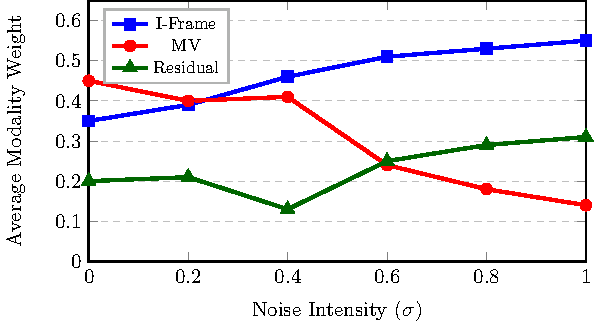
\includegraphics[width=\linewidth]{figure/figure3.pdf}
    \caption{Modality weight adaptation under MV noise injection.}
    \label{fig:noise_injection}
\end{minipage}\hfill
\begin{minipage}[t]{0.48\textwidth}
    \vspace{0pt} % 强制顶部对齐基线（解决图表错位的核心）
    \centering
    \begin{threeparttable}
        \caption{Ablative evaluation of Fusion Weight Module.}
        \label{tab:FusionWeight}
        \begin{tabular}{@{}lcc@{}}
        \toprule
        Fusion Weight & HMDB-51 & UCF-101 \\
        \midrule
        0: Fixed  & 75.9 & 96.4 \\
        1: Trainable & 76.0 & 96.5 \\
        2: IADF (Ours) & \textbf{76.2} & \textbf{96.7} \\
        \bottomrule
        \end{tabular}
    \end{threeparttable}
\end{minipage}

\vspace{0mm} % 上下两排间距

% ================= 第三排：Table 8 & Table 7 (移到最下，并左右调换) =================
\begin{minipage}[t]{0.48\textwidth}
    \vspace{0pt} % 强制顶部对齐基线
    \centering
    \begin{threeparttable}
        \caption{Ablative evaluation of Prompt configuration ablation.}
        \label{tab:prompt_ablation}
        \begin{tabular}{@{}lcc@{}}
        \toprule
        Strategy & HMDB-51 & UCF-101 \\
        \midrule
        w/o Dataset Name & 75.4 & 96.5 \\
        w/ Dataset Name & \textbf{76.2} & \textbf{96.7} \\
        \bottomrule
        \end{tabular}
    \end{threeparttable}
\end{minipage}\hfill
\begin{minipage}[t]{0.48\textwidth}
    \vspace{0pt} % 强制顶部对齐基线
    \centering
    \setlength{\tabcolsep}{2pt} 
    \begin{threeparttable}
        \caption{Comparison of inference time (ms) per video.}
        \label{tab:inferenceefficiency}
        \begin{tabular}{@{}lccc@{}}
        \toprule
        Method & \shortstack{Pre-\\process} & Inference & \shortstack{Full\\Pipeline} \\
        \midrule
        ActionCLIP~\cite{wang2021actionclipnewparadigmvideo} & 41.51 & \textbf{11.52} & 53.03 \\
        \methodname~(Ours) & \textbf{6.11} & 14.23 & \textbf{20.34} \\
        \bottomrule
        \end{tabular}
    \end{threeparttable}
\end{minipage}

\end{table}
\vspace{2mm} % 上下两排间距



\noindent\textbf{Effect of Attribute Generation Models.} Table~\ref{tab:attributewordgenerators} investigates the impact of different Large Language Models (LLMs) used for attribute generation. We compare Qwen3:8b and Llama3.1:8b, both generating $L=32$ attribute words using the same prompt. Results show that Llama3.1:8b achieves slightly better performance (\textbf{76.2\%} on HMDB-51 and \textbf{96.7\%} on UCF-101). The marginal difference indicates that our framework is robust to the choice of LLM, as both models can effectively capture action-relevant semantic attributes.

\noindent\textbf{Attribute Prompt Design.} Table~\ref{tab:attributeprompt} compares three textual supervision strategies: (0) class name only, (1) learnable prompt tokens~\cite{zhou2022learning}, and (2) our attribute-enhanced prompt. Results show clear progressive improvements: from 74.4\%/95.2\% (baseline) to 75.2\%/96.1\% (learnable tokens), and finally to 75.9\%/96.4\% (ours). This confirms that explicit, fine-grained semantic attributes provide richer supervision than standard class names or implicit learnable tokens.

\noindent\textbf{Effectiveness of Instance-Aware Dynamic Fusion (IADF).} Table~\ref{tab:FusionWeight} compares our module against fixed and trainable weight strategies. Compared to fixed (75.9\%/96.4\%) and naive trainable weights (76.0\%/96.5\%), our IADF achieves the highest accuracy (\textbf{76.2\%/96.7\%}). This demonstrates the effectiveness of using textual attributes to dynamically guide modality fusion.

\noindent\textbf{Robustness to Modality Noise.} To simulate interference, we add Gaussian noise $\mathcal{N}(0, \sigma^2)$ to the Motion Vector (MV) features during inference. As shown in Fig.~\ref{fig:noise_injection}, with increasing noise $\sigma$, our module dynamically drops the weight of the corrupted MV branch and elevates the I-frame and Residual branches. This confirms IADF can effectively isolate unreliable modalities to maintain robustness.

\noindent\textbf{Sensitivity to Attribute Quantity ($L$).} We explore the impact of the number of generated attributes ($L$). The performance peaks at $L=32$ (\textbf{76.2\%} on HMDB-51 and \textbf{96.7\%} on UCF-101). A smaller quantity ($L=16$) fails to capture sufficient fine-grained semantic diversity (75.6\%/96.4\%), while generating too many attributes ($L=64$) introduces semantic noise and redundancy, slightly degrading accuracy to 75.7\%/96.3\%.

\noindent\textbf{Impact of Dataset Context in Prompt.} Table~\ref{tab:prompt_ablation} highlights the importance of incorporating the dataset name into the LLM prompt template. By providing this context, the LLM generates domain-specific attributes tailored to the dataset's characteristics, yielding a noticeable improvement (\textbf{+0.8\%} on HMDB-51 and \textbf{+0.2\%} on UCF-101) compared to context-agnostic generation.

\noindent\textbf{Inference Efficiency Analysis.} We compare the inference efficiency of \methodname~with ActionCLIP~\cite{wang2021actionclipnewparadigmvideo} in Table~\ref{tab:inferenceefficiency}. ActionCLIP, processing raw video frames, requires a substantial 41.51 ms for video decoding pre-processing. By directly leveraging the compressed video stream, our method reduces pre-processing time by nearly 7$\times$ to only 6.11 ms. The full pipeline takes only \textbf{20.34 ms} per video, achieving a \textbf{2.6$\times$} speed-up over ActionCLIP's 53.03 ms, solidifying our model's superiority in real-world deployment efficiency.

\noindent\textbf{Qualitative Visualization.} As shown in Fig.~\ref{fig:attention_vis}, compared to fixed weight fusion, our IADF module demonstrates a clear advantage in focusing on dynamic action features. 

% 确保你的导言区包含了必要的宏包：
% \usepackage{graphicx}
% \usepackage{amsmath}

\begin{figure*}[t] % 使用 figure* 跨双栏显示。如果是单栏图，用 figure 即可。
    \centering
    % 【技巧1】定义统一的图片宽度，方便一键全局调整图片大小
    \newcommand{\imgw}{0.115\linewidth} 
    % 【技巧2】调整表格列间距（图片之间的水平间距）。设为0.5pt或0pt可以达到无缝拼接的效果
    \setlength{\tabcolsep}{1pt} 
    
    \begin{tabular}{c cccc c cccc}
        % 1. 顶部标题行
        & \multicolumn{4}{c}{Turn} 
        & % 这里留空，作为左右两组动作之间的分隔间距
        & \multicolumn{4}{c}{Hit} \\
        
        % 2. 第一行：I-Frames
        % \rotatebox{90} 用于将文字逆时针旋转90度
        \rotatebox{90}{\scriptsize I-Frames} & 
        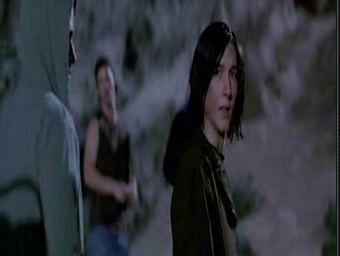
\includegraphics[width=\imgw]{figure/turn/turn_004_original.jpg} & 
        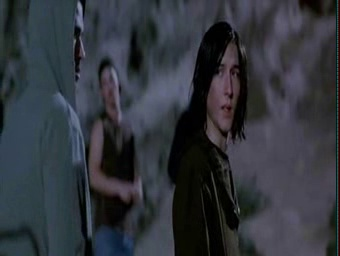
\includegraphics[width=\imgw]{figure/turn/turn_005_original.jpg} & 
        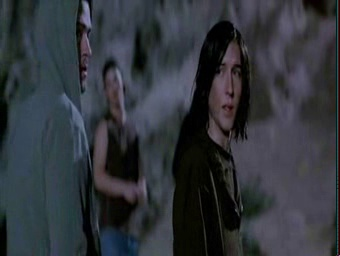
\includegraphics[width=\imgw]{figure/turn/turn_006_original.jpg} & 
        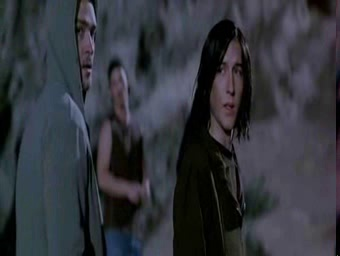
\includegraphics[width=\imgw]{figure/turn/turn_007_original.jpg} & 
        \quad & % 左右两组图片中间的较大空隙
        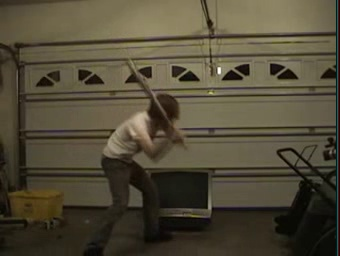
\includegraphics[width=\imgw]{figure/hit/hit_008_original.jpg} & 
        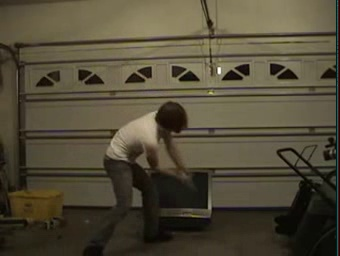
\includegraphics[width=\imgw]{figure/hit/hit_009_original.jpg} & 
        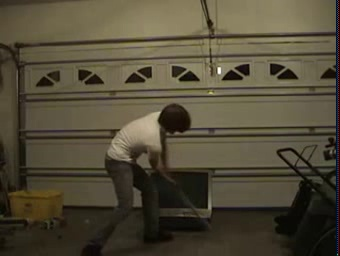
\includegraphics[width=\imgw]{figure/hit/hit_010_original.jpg} & 
        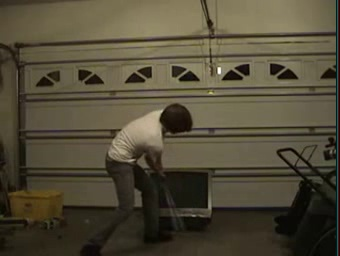
\includegraphics[width=\imgw]{figure/hit/hit_011_original.jpg} \\
        
        \\[-1.5mm] 
        
        % 3. 第二行：Attention
        \rotatebox{90}{\scriptsize coviar} & 
        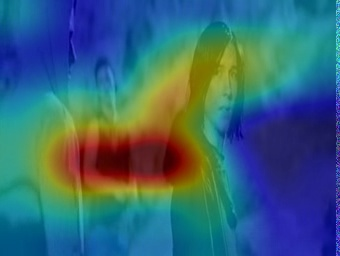
\includegraphics[width=\imgw]{figure/turn/turn_004_attention_c.jpg} & 
        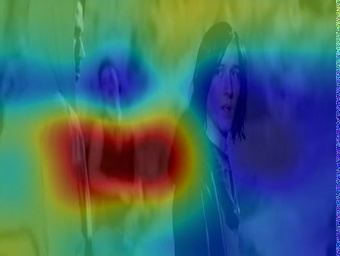
\includegraphics[width=\imgw]{figure/turn/turn_005_attention_c.jpg} & 
        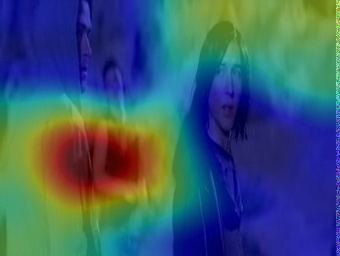
\includegraphics[width=\imgw]{figure/turn/turn_006_attention_c.jpg} & 
        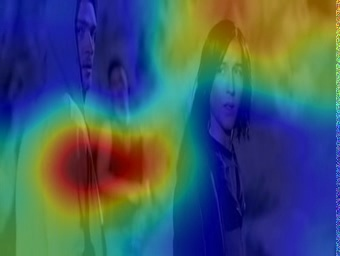
\includegraphics[width=\imgw]{figure/turn/turn_007_attention_c.jpg} & 
        \quad & % 保持和上一行相同的中间分隔
        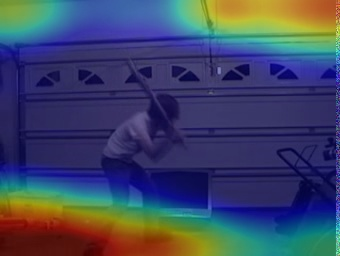
\includegraphics[width=\imgw]{figure/hit/hit_008_attention_c.jpg} & 
        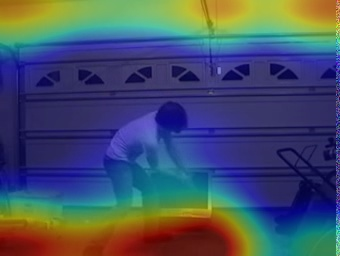
\includegraphics[width=\imgw]{figure/hit/hit_009_attention_c.jpg} & 
        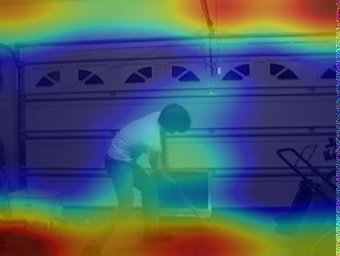
\includegraphics[width=\imgw]{figure/hit/hit_010_attention_c.jpg} & 
        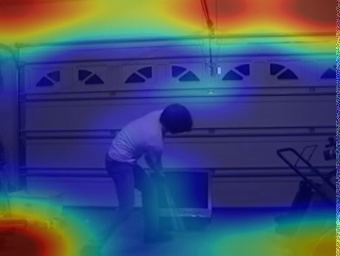
\includegraphics[width=\imgw]{figure/hit/hit_011_attention_c.jpg} \\
                % 【技巧3】使用 \\[-1.5mm] 来消除表格换行时的默认垂直间距，让上下两排图片贴紧
        \\[-1.5mm] 
        
        % 3. 第二行：Attention
        \rotatebox{90}{\scriptsize fix-weight} & 
        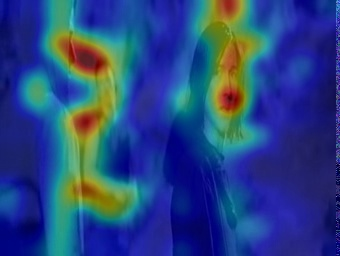
\includegraphics[width=\imgw]{figure/turn/turn_004_attention_p.jpg} & 
        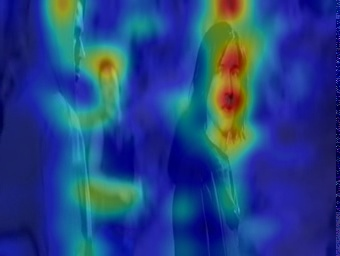
\includegraphics[width=\imgw]{figure/turn/turn_005_attention_p.jpg} & 
        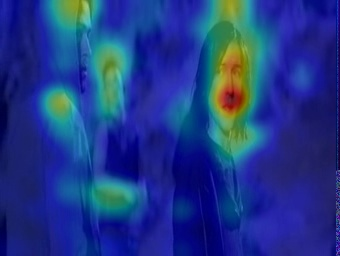
\includegraphics[width=\imgw]{figure/turn/turn_006_attention_p.jpg} & 
        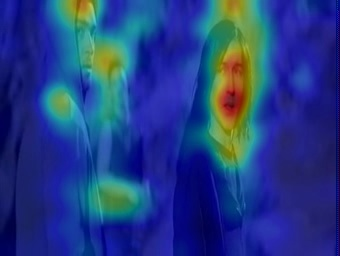
\includegraphics[width=\imgw]{figure/turn/turn_007_attention_p.jpg} & 
        \quad & % 保持和上一行相同的中间分隔
        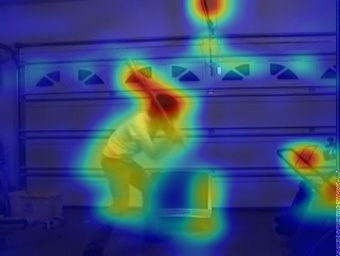
\includegraphics[width=\imgw]{figure/hit/hit_008_attention_p.jpg} & 
        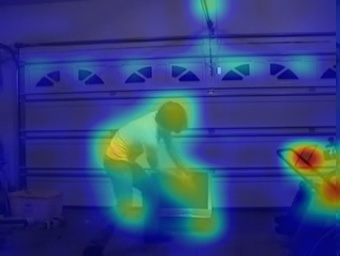
\includegraphics[width=\imgw]{figure/hit/hit_009_attention_p.jpg} & 
        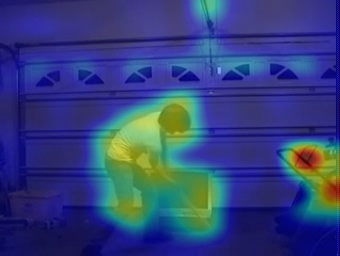
\includegraphics[width=\imgw]{figure/hit/hit_010_attention_p.jpg} & 
        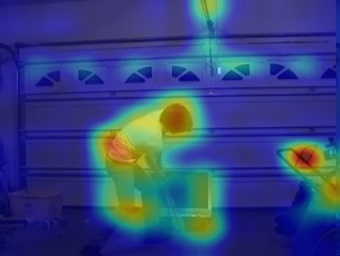
\includegraphics[width=\imgw]{figure/hit/hit_011_attention_p.jpg} \\
                % 【技巧3】使用 \\[-1.5mm] 来消除表格换行时的默认垂直间距，让上下两排图片贴紧
        \\[-1.5mm] 
        
        % 3. 第二行：Attention
        \rotatebox{90}{\scriptsize IADF} & 
        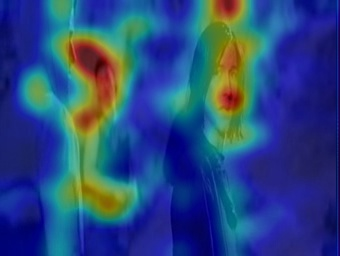
\includegraphics[width=\imgw]{figure/turn/turn_004_attention_f.jpg} & 
        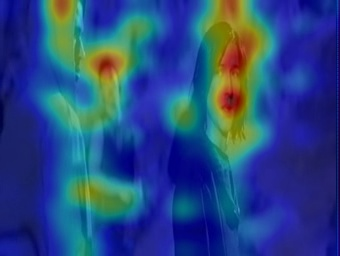
\includegraphics[width=\imgw]{figure/turn/turn_005_attention_f.jpg} & 
        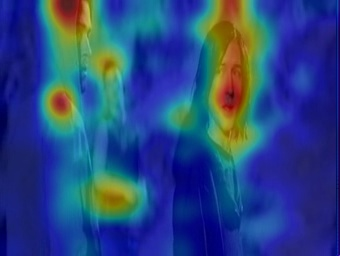
\includegraphics[width=\imgw]{figure/turn/turn_006_attention_f.jpg} & 
        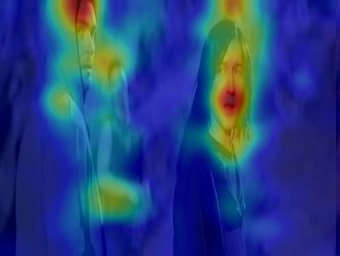
\includegraphics[width=\imgw]{figure/turn/turn_007_attention_f.jpg} & 
        \quad & % 保持和上一行相同的中间分隔
        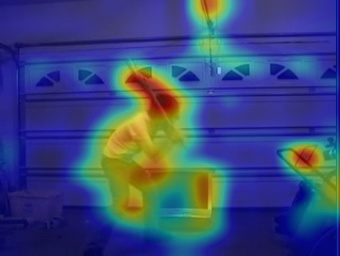
\includegraphics[width=\imgw]{figure/hit/hit_008_attention_f.jpg} & 
        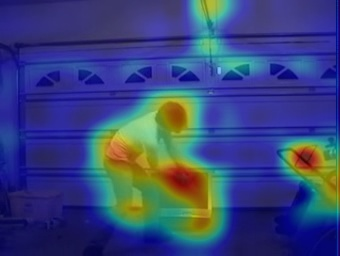
\includegraphics[width=\imgw]{figure/hit/hit_009_attention_f.jpg} & 
        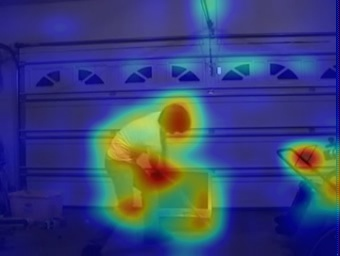
\includegraphics[width=\imgw]{figure/hit/hit_010_attention_f.jpg} & 
        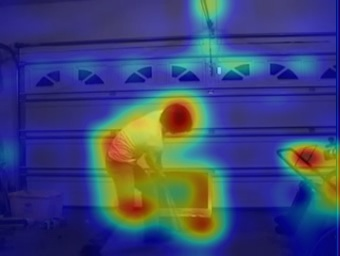
\includegraphics[width=\imgw]{figure/hit/hit_011_attention_f.jpg} \\
                % 【技巧3】使用 \\[-1.5mm] 来消除表格换行时的默认垂直间距，让上下两排图片贴紧
    \end{tabular}
    
    % 可选：微调Caption和图片之间的距离
    \vspace{-2mm} 
    \caption{Visualization of attention maps from HMDB-51.}
    \label{fig:attention_vis}
\end{figure*}


\section{Conclusions}
\label{sec:conclusion}
In this paper, we proposed TextComp, a novel framework that bridges the semantic gap in compressed video action recognition via text-guided navigation. By leveraging Large Language Models (LLMs) to decompose action categories into multifaceted semantic attributes. To fully exploit these textual priors without collapsing pre-trained feature spaces, we designed the Instance-Aware Dynamic Fusion (IADF) module, which adaptively routes visual features based on semantic queries. Extensive experiments across four benchmarks demonstrate that TextComp effectively balances computational efficiency and high recognition accuracy, consistently outperforming existing compressed-domain methods. These results validate the immense potential of vision-language synergy in resource-constrained video understanding.



\clearpage

\bibliographystyle{splncs04}
\bibliography{egbib}
\end{document}
